% GNUPLOT: LaTeX picture with Postscript
\begingroup
  % Encoding inside the plot.  In the header of your document, this encoding
  % should to defined, e.g., by using
  % \usepackage[cp1252,<other encodings>]{inputenc}
  \inputencoding{cp1252}%
  \makeatletter
  \providecommand\color[2][]{%
    \GenericError{(gnuplot) \space\space\space\@spaces}{%
      Package color not loaded in conjunction with
      terminal option `colourtext'%
    }{See the gnuplot documentation for explanation.%
    }{Either use 'blacktext' in gnuplot or load the package
      color.sty in LaTeX.}%
    \renewcommand\color[2][]{}%
  }%
  \providecommand\includegraphics[2][]{%
    \GenericError{(gnuplot) \space\space\space\@spaces}{%
      Package graphicx or graphics not loaded%
    }{See the gnuplot documentation for explanation.%
    }{The gnuplot epslatex terminal needs graphicx.sty or graphics.sty.}%
    \renewcommand\includegraphics[2][]{}%
  }%
  \providecommand\rotatebox[2]{#2}%
  \@ifundefined{ifGPcolor}{%
    \newif\ifGPcolor
    \GPcolortrue
  }{}%
  \@ifundefined{ifGPblacktext}{%
    \newif\ifGPblacktext
    \GPblacktexttrue
  }{}%
  % define a \g@addto@macro without @ in the name:
  \let\gplgaddtomacro\g@addto@macro
  % define empty templates for all commands taking text:
  \gdef\gplbacktext{}%
  \gdef\gplfronttext{}%
  \makeatother
  \ifGPblacktext
    % no textcolor at all
    \def\colorrgb#1{}%
    \def\colorgray#1{}%
  \else
    % gray or color?
    \ifGPcolor
      \def\colorrgb#1{\color[rgb]{#1}}%
      \def\colorgray#1{\color[gray]{#1}}%
      \expandafter\def\csname LTw\endcsname{\color{white}}%
      \expandafter\def\csname LTb\endcsname{\color{black}}%
      \expandafter\def\csname LTa\endcsname{\color{black}}%
      \expandafter\def\csname LT0\endcsname{\color[rgb]{1,0,0}}%
      \expandafter\def\csname LT1\endcsname{\color[rgb]{0,1,0}}%
      \expandafter\def\csname LT2\endcsname{\color[rgb]{0,0,1}}%
      \expandafter\def\csname LT3\endcsname{\color[rgb]{1,0,1}}%
      \expandafter\def\csname LT4\endcsname{\color[rgb]{0,1,1}}%
      \expandafter\def\csname LT5\endcsname{\color[rgb]{1,1,0}}%
      \expandafter\def\csname LT6\endcsname{\color[rgb]{0,0,0}}%
      \expandafter\def\csname LT7\endcsname{\color[rgb]{1,0.3,0}}%
      \expandafter\def\csname LT8\endcsname{\color[rgb]{0.5,0.5,0.5}}%
    \else
      % gray
      \def\colorrgb#1{\color{black}}%
      \def\colorgray#1{\color[gray]{#1}}%
      \expandafter\def\csname LTw\endcsname{\color{white}}%
      \expandafter\def\csname LTb\endcsname{\color{black}}%
      \expandafter\def\csname LTa\endcsname{\color{black}}%
      \expandafter\def\csname LT0\endcsname{\color{black}}%
      \expandafter\def\csname LT1\endcsname{\color{black}}%
      \expandafter\def\csname LT2\endcsname{\color{black}}%
      \expandafter\def\csname LT3\endcsname{\color{black}}%
      \expandafter\def\csname LT4\endcsname{\color{black}}%
      \expandafter\def\csname LT5\endcsname{\color{black}}%
      \expandafter\def\csname LT6\endcsname{\color{black}}%
      \expandafter\def\csname LT7\endcsname{\color{black}}%
      \expandafter\def\csname LT8\endcsname{\color{black}}%
    \fi
  \fi
    \setlength{\unitlength}{0.0500bp}%
    \ifx\gptboxheight\undefined%
      \newlength{\gptboxheight}%
      \newlength{\gptboxwidth}%
      \newsavebox{\gptboxtext}%
    \fi%
    \setlength{\fboxrule}{0.5pt}%
    \setlength{\fboxsep}{1pt}%
\begin{picture}(9070.00,4534.00)%
    \gplgaddtomacro\gplbacktext{%
      \csname LTb\endcsname%%
      \put(682,930){\makebox(0,0)[r]{\strut{}2}}%
      \put(682,1381){\makebox(0,0)[r]{\strut{}4}}%
      \put(682,1832){\makebox(0,0)[r]{\strut{}6}}%
      \put(682,2283){\makebox(0,0)[r]{\strut{}8}}%
      \put(682,2734){\makebox(0,0)[r]{\strut{}10}}%
      \put(682,3185){\makebox(0,0)[r]{\strut{}15}}%
      \put(682,3636){\makebox(0,0)[r]{\strut{}20}}%
      \put(682,4087){\makebox(0,0)[r]{\strut{}25}}%
      \put(1052,484){\makebox(0,0){\strut{}1e-06}}%
      \put(1528,484){\makebox(0,0){\strut{}1e-05}}%
      \put(2004,484){\makebox(0,0){\strut{}0.0001}}%
      \put(2480,484){\makebox(0,0){\strut{}0.001}}%
      \put(2956,484){\makebox(0,0){\strut{}0.01}}%
      \put(3432,484){\makebox(0,0){\strut{}0.1}}%
      \put(3908,484){\makebox(0,0){\strut{}0.5}}%
      \put(4383,484){\makebox(0,0){\strut{}1}}%
      \put(4859,484){\makebox(0,0){\strut{}2}}%
      \put(5335,484){\makebox(0,0){\strut{}5}}%
      \put(5811,484){\makebox(0,0){\strut{}10}}%
      \put(6287,484){\makebox(0,0){\strut{}50}}%
      \put(6763,484){\makebox(0,0){\strut{}100}}%
      \put(7239,484){\makebox(0,0){\strut{}1000}}%
    }%
    \gplgaddtomacro\gplfronttext{%
      \csname LTb\endcsname%%
      \put(209,2508){\rotatebox{-270}{\makebox(0,0){\strut{}$m$ (memory)}}}%
      \put(4145,154){\makebox(0,0){\strut{}$\beta$ (relaxation)}}%
      \csname LTb\endcsname%%
      \put(8109,1190){\makebox(0,0)[l]{\strut{}$0.001$}}%
      \put(8109,2657){\makebox(0,0)[l]{\strut{}$0.01$}}%
      \put(8109,4125){\makebox(0,0)[l]{\strut{}$0.1$}}%
      \put(8835,2508){\rotatebox{-270}{\makebox(0,0){\strut{}Time taken ($s$)}}}%
    }%
    \gplbacktext
    \put(0,0){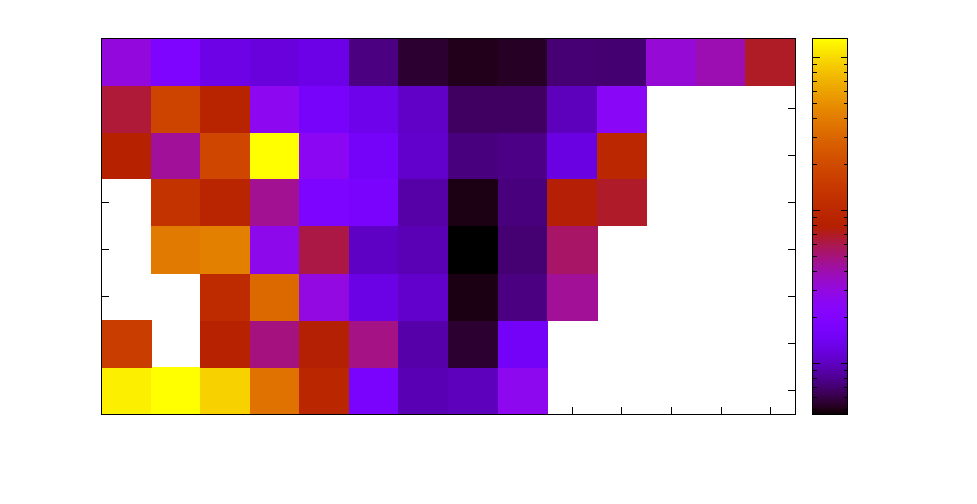
\includegraphics{heat_map}}%
    \gplfronttext
  \end{picture}%
\endgroup
